\section*{Annexes}
\phantomsection\addcontentsline{toc}{section}{Annexes}

\subsection*{Annexe 1 - Lexique}


Disponible à l'addresse: \url{https://github.com/LiberTIC/ODEV2/blob/master/doc/Thibaud_Printemps2015/lexique.md}


\subsubsection*{Protocoles}

\underline{\textbf{WebDAV}} (ou \textbf{Web Distributed Authoring and Versioning}) est une extension du protocol \textbf{HTTP}. Il permet de récupérer, déposer, synchronier et publier des fichiers rapidement et facilement. WebDAV permet une édition de contenu simultanée avec plusieurs utilisateurs. WebDAV est décrit dans la RFC 4918\rf{RFC4918}.

\textit{Source: \blurl{http://en.wikipedia.org/wiki/WebDAV}{Wikipédia - WebDAV}}\\

\underline{\textbf{CalDAV}} (ou \textbf{Calendar Extensions to WebDAV}) est est un standard internet permettant à un client de planifier des informations sur un serveur distant. Il étend les spécifications de \textbf{WebDAV} et utilise le format \textbf{iCalendar} pour les données. CalDAV est décrit dans la RFC 4791\rf{RFC4791}.

\textit{Source: \blurl{http://en.wikipedia.org/wiki/CalDAV}{Wikipédia - CalDAV}}\\

\underline{\textbf{CardDAV}} (ou \textbf{vCard Extensions to WebDAV}) est un standard internet permettant à un client d'accéder et de partager des données de contacts sur un serveur disant. Il étend les spécifications de \textbf{WebDAV} et utilise le format \textbf{vCard} pour les données. CardDAV est décrit dans le RFC 6352\rf{RFC6352}.

\textit{Source: \blurl{http://en.wikipedia.org/wiki/CardDAV}{Wikipédia - CardDAV}}\\


\subsubsection*{Formats de fichiers}

\underline{\textbf{iCalendar}} est un format de fichier (.ical ; .ics ; .ifb ; .icalendar) permettant d'envoyer des événements entre utilisateur. iCalendar est indépendant du protocol de transport. En effet, le transport eut être effectué par mail, par partage sur un serveur \textbf{WebDAV} ou même par pigeon voyageur. iCalendar est décrit dans la RFC 5545\rf{RFC5545}.

\textit{Source: \blurl{http://en.wikipedia.org/wiki/ICalendar}{Wikipédia - iCalendar}}\\

\underline{\textbf{vCard}} est un format de fichier (.vcf ; .vcard) permettant de de transmettre des données personnelles (sous forme de Carte de visite). Le format vCal peut être utilisé en parallèle avec le format \textbf{iCalendar} pour lier des événements à des personnes. vCard est décrit dans la RFC 6350\rf{rfc6350}. La version actuelle est la 4.0, mais la 3.0 reste utilisé par de nombreux clients et serveurs.

\textit{Source: \blurl{http://en.wikipedia.org/wiki/VCard}{Wikipédia - vCard}}\\

\underline{\textbf{hCalendar}} (ou \textbf{HTML iCalendar}) est un microformat pour afficher une représentation HTML sémantique d'un calendrier au format iCalendar. L'avantage, outre un affichage personnalisé des événements, est la possibilité données à des outils de parsing d'extraire les informations pour les stocker sous le format souhaité (iCalendar ou autre). hCalendar est utilisé entre autres par Facebook, Google et Wikipédia.

\textit{Source: \blurl{http://en.wikipedia.org/wiki/HCalendar}{Wikipédia - hCalendar}}\\

\underline{\textbf{jCal}} est une spécification de format JSON pour iCalendar. Il permet de stocker les données décrit par iCalendar sous le format JSON. Il est défini par la RFC 7265\rf{rfc7265}. Cependant, cette RFC n'est qu'une proposition de standard, émise en mai 2014: elle peux donc évoluer.

\textit{Source: \blurl{https://tools.ietf.org/html/rfc7265}{IETF - RFC 7265}}\\


\subsubsection*{Clients}

\underline{\textbf{iCal}} (renommé \textbf{Apple Calendar} depuis OSX Mountain Lion) est l'application de gestion de calendrier fait par Apple. Il peux entre autres, être client d'un serveur \textbf{WebDAV}.

\textit{Source: \blurl{http://en.wikipedia.org/wiki/Calendar_\%28application\%29}{Wikipédia - Calendar}}\\


\subsubsection*{Serveurs}

\underline{\textbf{SabreDAV}} est un serveur \textbf{CardDAV}, \textbf{CalDAV} et \textbf{WebDAV}. Il implémente les recommendations RFC actuelles. Il est compatible avec toutes les plateformes majeures.

\textit{Source: \blurl{http://en.wikipedia.org/wiki/SabreDAV}{Wikipédia - SabreDAV}}\\

\underline{\textbf{CalServ}}, aussi appelé \textbf{Calendars and Contacts Server} ou \textbf{Calendar Server} est un projet d'Apple d'implémentation des protocoles CalDAV et CardDAV. Sortie en 2006 sous le nom de iCal Server and Address Book Server, il a été porté sur des plateformes non-Apple. Il est écrit en Python et utilise une base de données SQL pour stocker les données.

\textit{Source: \blurl{http://en.wikipedia.org/wiki/Calendar_and_Contacts_Server}{Wikipédia - Calendar Server}}\\


\subsubsection*{Mix}

\underline{\textbf{Baïkal}} est une surcouche de SabreDAV. Il propose entre autres une interface d'administration web permettant la gestion du serveur CalDAV et CardDAV. Il est donc serveur et client de son propre serveur.

\textit{Source: \blurl{http://baikal-server.com/}{Site Baïkal}}

\clearpage

\subsection*{Annexe 2 - Modèle Evénement}

Disponible à l'addresse: \url{https://github.com/LiberTIC/ODEV2/blob/master/doc/Thibaud_Printemps2015/Modele_Evenement.md}

\begin{table}[h]
\begin{adjustwidth}{-1.8cm}{}
\begin{tabular}{|l || c | l | l | l |}

\hline
{\bf Propriété}&{\bf Type}&{\bf Description}&{\bf Source}&{\bf Exemple}\\
\hline
\hline

{\bf Base} &  &  &  &  \\

Nom & Texte & Nom court de l'événement & iCalendar & Concert Shakaponk \\
UID & Nombre & Identifiant Unique de l'event & iCalendar & SL-2015-XYZ-004 \\
Description & Texte & Description de l'événement & iCalendar & Concert de rock avec {[}...{]} \\

\hline

{\bf Date et heure} &  &  &  &  \\

Date début & Date & Date et heure de début & iCalendar & 2015-06-20 / 20:00 \\
Date fin & Date & Date et heure de fin & iCalendar & 2015-06-20 / 23:30 \\
Date création & Date & Date de création de l'event & ODE\_V2 & 2015-04-01 / 13:37 \\
Date modification & Date & Date de modif de l'événement & ODE\_V2 & 2015-04-03 / 20:15 \\

\hline

{\bf Localisation} &  &  &  &  \\

Lieu & Texte & Nom de l'endroit & iCalendar & Zénith Nantes \\
Emplacement & Texte & Nom de l'endroit & ODE\_V2 & Salle de concert \#3 \\
Géolocalisation & Geo & Géolocalisation de l'événement & iCalendar & 47.229234, -1.628550 \\
Capacité du lieu & Nombre & Capacité du lieu de l'event & ODE\_V1 & 4000 (personnes) \\

\hline

{\bf Organisation} &  &  &  &  \\

Participants & Texte & Participants à l'événement & schema.org & Shakaponk;Tagada Jones \\
Durée & Durée & Durée de l'événement & schema.org & PT3H30M (3h30min) \\
Status & Texte & Status de l'événement & iCalendar & Annulé / Reporté \\
Organisateur & Texte & Organisateur de l'événement & schema.org & Stéréolux \\
Sous-Evénement & UID & UID d'un sous-événement & schema.org & SL-2015-XYZ-009 \\
Super-Evénement & UID & UID d'un sur-événement & schema.org & SL-2015-XYZ-001 \\

\hline

{\bf URLs} &  &  &  &  \\

URL & URL & URL vers le site ODEV2 & iCalendar & http://ODEV2/event/XYZ004 \\
URL orga & URL & URL de l'event sur le site de l'orga & schema.org & http://stereolux/event/XYZ004 \\
URLs médias & URLs & URL de média compatible oEmbed & schema.org & http://website/image.jpg \\

\hline

{\bf International} &  &  &  &  \\

Langue & Texte & Langue de l'événement & ODE\_V1 & FR \\

\hline

{\bf Tarifs} &  &  &  &  \\

Prix standard & Nombre & Prix au tarif normal & ODE\_V2 & 10 \\
Prix réduit & Nombre & Prix au tarif réduit & ODE\_V2 & 7.5 \\
Prix enfant & Nombre & Prix au tarif enfant & ODE\_V2 & 5 \\

\hline

{\bf Contacts} & &  &  &  \\

Contact - Nom & Texte & Nom du contact & ODE\_V1 & John Smith \\
Contact - Email & Email & Email du contact & ODE\_V1 & john.smith@email.com \\

\hline

{\bf Catégorisation} & &  &  &  \\

Catégorie & Texte & Catégorie de l'événement & ODE\_V1 & Concert \\
Tags & Texte & Tags de l'événement & ODE\_V1 & Rock;Alternatif;{[}...{]} \\

\hline

\end{tabular}
\end{adjustwidth}
\end{table}

\subsection*{Annexe 3 - Diagramme de Cas d'Utilisation}

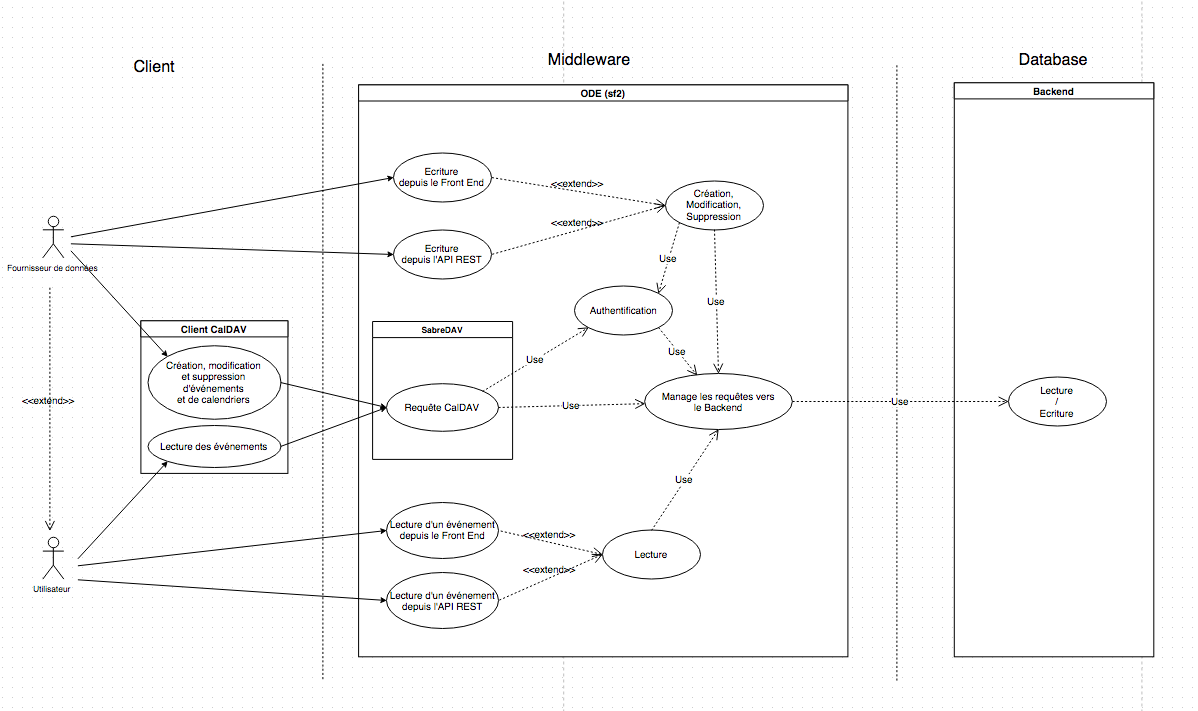
\includegraphics[angle=90,origin=c,height=190mm]{diagramme_cas_utilisation.png}